\documentclass[11pt,openany]{book}

\usepackage[T1]{fontenc}
\usepackage[utf8]{inputenc}
\usepackage{lmodern}
\usepackage{geometry}
\geometry{paper=letterpaper,inner=1.05in,outer=0.85in,top=0.85in,bottom=0.9in}
\usepackage{microtype}
\DisableLigatures{encoding = *, family = tt*}
\usepackage{xcolor}
\usepackage{graphicx}
\usepackage{tikz}
\usetikzlibrary{arrows.meta,calc,positioning,shapes.geometric}
\usepackage{booktabs}
\usepackage{longtable}
\usepackage{tabularx}
\usepackage{array}
\usepackage{enumitem}
\usepackage{listings}
\usepackage[most]{tcolorbox}
\usepackage{fancyhdr}
\usepackage{titlesec}
\usepackage{hyperref}
\usepackage{bookmark}

\definecolor{voidblack}{HTML}{090B10}
\definecolor{hull}{HTML}{161C27}
\definecolor{steel}{HTML}{5F6B7A}
\definecolor{ash}{HTML}{D8DCE3}
\definecolor{signalred}{HTML}{A92C35}
\definecolor{ember}{HTML}{E35D4F}
\definecolor{plasma}{HTML}{7FB7BE}
\definecolor{codeback}{HTML}{F2F4F7}
\definecolor{linkblue}{HTML}{245E78}

\hypersetup{
  colorlinks=true,
  linkcolor=signalred,
  urlcolor=linkblue,
  citecolor=linkblue,
  pdftitle={Blackship: Technical Manual},
  pdfauthor={The Blackship contributors},
  pdfsubject={FreeBSD jail orchestration},
  pdfkeywords={FreeBSD, jails, ZFS, VNET, PF, orchestration}
}

\titleformat{\chapter}[display]
  {\normalfont\bfseries\color{voidblack}}
  {\filleft\Large\color{signalred}\MakeUppercase{\chaptertitlename}\ \thechapter}
  {1ex}
  {\titlerule\vspace{1.2ex}\Huge}
\titleformat{\section}{\Large\bfseries\color{voidblack}}{\thesection}{0.7em}{}
\titleformat{\subsection}{\large\bfseries\color{signalred}}{\thesubsection}{0.7em}{}

\pagestyle{fancy}
\fancyhf{}
\fancyhead[LE]{\small\scshape Blackship Technical Manual}
\fancyhead[RO]{\small\scshape\nouppercase{\leftmark}}
\fancyfoot[C]{\thepage}
\renewcommand{\headrulewidth}{0.4pt}
\renewcommand{\footrulewidth}{0pt}
\setlength{\headheight}{14pt}

\setlist{nosep,leftmargin=1.5em}
\setlength{\parindent}{0pt}
\setlength{\parskip}{0.65em}
\renewcommand{\arraystretch}{1.15}
\emergencystretch=2em

\lstdefinelanguage{TOML}{
  sensitive=true,
  morecomment=[l]{\#},
  morestring=[b]",
  alsoletter={-},
  morekeywords={true,false}
}
\lstdefinelanguage{Jailfile}{
  sensitive=true,
  morecomment=[l]{\#},
  morekeywords={FROM,LABEL,ARG,ENV,RUN,COPY,WORKDIR,EXPOSE,CMD,STOP}
}
\lstdefinelanguage{JSON}{
  sensitive=true,
  morestring=[b]",
  morecomment=[l]{//},
  morekeywords={true,false,null}
}
\lstdefinelanguage{Rust}{
  sensitive=true,
  morecomment=[l]{//},
  morecomment=[s]{/*}{*/},
  morestring=[b]",
  morekeywords={as,async,await,break,const,continue,crate,dyn,else,enum,extern,
    false,fn,for,if,impl,in,let,loop,match,mod,move,mut,pub,ref,return,self,
    Self,static,struct,super,trait,true,type,unsafe,use,where,while}
}
\lstset{
  basicstyle=\ttfamily\small,
  backgroundcolor=\color{codeback},
  frame=single,
  rulecolor=\color{steel!55},
  breaklines=true,
  breakatwhitespace=false,
  keepspaces=true,
  columns=fullflexible,
  showstringspaces=false,
  keywordstyle=\bfseries\color{signalred},
  commentstyle=\itshape\color{steel},
  stringstyle=\color{linkblue},
  numbers=none,
  xleftmargin=0.4em,
  xrightmargin=0.4em,
  aboveskip=0.8em,
  belowskip=0.8em
}

\newtcolorbox{shipnote}[1][Note]{
  enhanced,
  breakable,
  colback=plasma!8,
  colframe=plasma!65!black,
  title=\textbf{#1},
  coltitle=white,
  fonttitle=\bfseries,
  boxrule=0.7pt,
  arc=1pt
}
\newtcolorbox{shipwarning}[1][Caution]{
  enhanced,
  breakable,
  colback=ember!7,
  colframe=signalred,
  title=\textbf{#1},
  coltitle=white,
  fonttitle=\bfseries,
  boxrule=0.8pt,
  arc=1pt
}

\newcommand{\command}[1]{\texttt{#1}}
\newcommand{\file}[1]{\path{#1}}
\newcommand{\setting}[1]{\texttt{#1}}
\newcommand{\Blackship}{\textsc{Blackship}}
\newcolumntype{Y}{>{\raggedright\arraybackslash}X}
\newcolumntype{L}[1]{>{\raggedright\arraybackslash}p{#1}}


\newcommand{\BlackshipVersion}{0.3.0}
\newcommand{\ManualEdition}{First edition}

\begin{document}

\frontmatter
\begin{titlepage}
\thispagestyle{empty}
\begin{tikzpicture}[remember picture,overlay]
  % Deep-space ground with a restrained cold glow behind the vessel.
  \shade[top color=voidblack,bottom color=black]
    (current page.south west) rectangle (current page.north east);
  \begin{scope}[shift={($(current page.center)+(0,-0.65cm)$)}]
    \shade[inner color=plasma!18,outer color=voidblack,opacity=0.72]
      (0,0.2) ellipse (7.1cm and 5.3cm);
    \draw[plasma!18,opacity=0.28,line width=0.55pt]
      (-7.4,-1.8) .. controls (-3.8,1.2) and (3.3,-3.0) .. (7.5,0.9);
    \draw[steel!35,opacity=0.18,line width=1.1pt]
      (-7.0,-2.4) .. controls (-2.7,0.4) and (2.5,-2.5) .. (7.1,1.4);

    % A half-lit world gives the silhouette depth without external artwork.
    \fill[steel!22,opacity=0.62] (4.9,2.3) circle (2.05cm);
    \fill[voidblack] (5.55,2.72) circle (2.02cm);
    \draw[plasma!35,opacity=0.55,line width=0.65pt]
      (4.9,0.25) arc[start angle=-90,end angle=90,radius=2.05cm];
  \end{scope}

  % Deterministic star field: reproducible and sharp at any resolution.
  \foreach \x/\y/\r/\o in {
    0.05/0.91/0.45/0.55,0.11/0.78/0.75/0.80,0.17/0.88/0.35/0.65,
    0.23/0.70/0.45/0.70,0.29/0.95/0.60/0.75,0.35/0.81/0.35/0.50,
    0.42/0.91/0.75/0.85,0.49/0.75/0.40/0.60,0.56/0.94/0.35/0.55,
    0.63/0.83/0.62/0.80,0.70/0.90/0.42/0.65,0.78/0.73/0.72/0.82,
    0.85/0.96/0.42/0.70,0.92/0.84/0.35/0.60,0.97/0.68/0.62/0.78,
    0.08/0.61/0.35/0.50,0.15/0.51/0.52/0.70,0.24/0.63/0.34/0.55,
    0.76/0.59/0.43/0.62,0.87/0.50/0.62/0.75,0.95/0.61/0.34/0.55,
    0.04/0.34/0.60/0.72,0.12/0.24/0.34/0.52,0.20/0.39/0.45/0.62,
    0.31/0.28/0.32/0.50,0.69/0.32/0.34/0.55,0.80/0.20/0.55/0.72,
    0.91/0.39/0.34/0.52,0.61/0.16/0.45/0.65,0.38/0.18/0.30/0.48}
    \fill[ash,opacity=\o]
      ([xshift=\x\paperwidth,yshift=\y\paperheight]current page.south west)
      circle (\r pt);

  % Original gothic voidship: a vertical ark built from layered vector forms.
  \begin{scope}[shift={($(current page.center)+(0,-0.75cm)$)},scale=0.93,
      line join=round,line cap=round]
    % Engine bloom and the massive outer silhouette.
    \shade[inner color=plasma!80,outer color=voidblack,opacity=0.62]
      (0,-4.55) ellipse (1.85cm and 1.0cm);
    \fill[black,opacity=0.72]
      (0,4.72) -- (-0.68,3.72) -- (-1.32,3.10) -- (-1.62,1.92) --
      (-2.72,1.08) -- (-3.58,0.72) -- (-4.48,-0.18) -- (-3.58,-0.58) --
      (-2.85,-1.38) -- (-2.48,-3.62) -- (-1.25,-4.48) -- (0,-5.08) --
      (1.25,-4.48) -- (2.48,-3.62) -- (2.85,-1.38) -- (3.58,-0.58) --
      (4.48,-0.18) -- (3.58,0.72) -- (2.72,1.08) -- (1.62,1.92) --
      (1.32,3.10) -- (0.68,3.72) -- cycle;

    % Armoured wings and layered prow.
    \fill[hull]
      (0,4.40) -- (-0.56,3.52) -- (-1.08,2.86) -- (-1.28,1.48) --
      (-2.35,0.70) -- (-3.92,-0.12) -- (-2.64,-0.58) -- (-2.16,-1.28) --
      (-1.86,-3.42) -- (-0.92,-4.12) -- (0,-4.55) --
      (0.92,-4.12) -- (1.86,-3.42) -- (2.16,-1.28) -- (2.64,-0.58) --
      (3.92,-0.12) -- (2.35,0.70) -- (1.28,1.48) -- (1.08,2.86) --
      (0.56,3.52) -- cycle;
    \fill[steel!28!hull]
      (-3.86,-0.12) -- (-1.34,1.25) -- (-1.58,0.18) -- (-2.62,-0.62) -- cycle;
    \fill[steel!28!hull]
      (3.86,-0.12) -- (1.34,1.25) -- (1.58,0.18) -- (2.62,-0.62) -- cycle;
    \draw[steel!68,line width=0.55pt]
      (-3.72,-0.12) -- (-1.40,0.98) -- (-0.94,3.05) -- (0,4.20) --
      (0.94,3.05) -- (1.40,0.98) -- (3.72,-0.12);

    % Cathedral nave, buttresses, and needle-like towers.
    \fill[voidblack]
      (0,3.86) -- (-0.48,2.85) -- (-0.62,-2.94) -- (0,-4.12) --
      (0.62,-2.94) -- (0.48,2.85) -- cycle;
    \fill[steel!38!hull]
      (0,3.55) -- (-0.30,2.70) -- (-0.34,-2.68) -- (0,-3.54) --
      (0.34,-2.68) -- (0.30,2.70) -- cycle;
    \foreach \s in {-1,1}{
      \fill[hull] ({\s*0.70},2.08) -- ({\s*1.02},3.22) --
        ({\s*1.20},1.62) -- ({\s*0.92},0.68) -- cycle;
      \fill[hull] ({\s*1.08},0.62) -- ({\s*1.62},2.02) --
        ({\s*1.76},0.34) -- ({\s*1.38},-0.78) -- cycle;
      \fill[hull] ({\s*1.34},-0.88) -- ({\s*2.05},0.02) --
        ({\s*2.20},-1.60) -- ({\s*1.68},-2.62) -- cycle;
      \draw[steel!58,line width=0.45pt]
        ({\s*0.72},2.02) -- ({\s*1.16},1.47) -- ({\s*0.92},0.60);
      \draw[steel!58,line width=0.45pt]
        ({\s*1.10},0.54) -- ({\s*1.70},0.08) -- ({\s*1.36},-0.84);
      \draw[steel!58,line width=0.45pt]
        ({\s*1.36},-0.94) -- ({\s*2.12},-1.50) -- ({\s*1.66},-2.55);
    }

    % Ribbed armour, lancet windows, and restrained signal lighting.
    \foreach \y/\w in {2.42/0.82,1.70/1.08,0.98/1.34,0.26/1.52,
        -0.46/1.48,-1.18/1.30,-1.90/1.08,-2.62/0.82}
      \draw[steel!48,line width=0.42pt] (-\w,\y) -- (0,\y-0.20) -- (\w,\y);
    \foreach \y in {2.35,1.76,1.17,0.58,-0.01,-0.60,-1.19,-1.78,-2.37}
      \fill[plasma!85] (0,\y) ellipse (1.05pt and 2.15pt);
    \draw[signalred!82,line width=0.75pt]
      (-0.80,-3.18) -- (0,-3.56) -- (0.80,-3.18);

    % Engine housings and cold exhaust apertures.
    \foreach \x in {-1.10,-0.55,0,0.55,1.10}{
      \fill[black] (\x,-3.82) ellipse (0.25cm and 0.46cm);
      \fill[plasma!75] (\x,-4.02) ellipse (0.13cm and 0.30cm);
      \fill[white,opacity=0.65] (\x,-4.08) ellipse (0.045cm and 0.15cm);
    }
    \draw[plasma!45,opacity=0.75,line width=0.6pt]
      (-0.82,-4.32) .. controls (-0.50,-4.72) and (-0.20,-4.84) .. (0,-4.92)
      .. controls (0.20,-4.84) and (0.50,-4.72) .. (0.82,-4.32);
  \end{scope}

  \fill[plasma!65!black] (current page.south west)
    rectangle ($(current page.south east)+(0,0.12cm)$);
\end{tikzpicture}

\vspace*{0.70in}
\begin{center}
  {\fontsize{42}{46}\selectfont\bfseries\color{ash} BLACKSHIP}\par
  \vspace{0.16in}
  {\Large\color{plasma}\MakeUppercase{Technical Manual}}\par
  \vspace{0.10in}
  {\large\color{steel!45!white} FreeBSD Jail Orchestration}\par
\end{center}

\vfill
\begin{center}
  {\large\color{ash} Version \BlackshipVersion}\par
  \vspace{0.10in}
  {\small\color{steel!35!white} \ManualEdition\quad---\quad November 2026}\par
\end{center}
\vspace*{0.42in}
\end{titlepage}

\thispagestyle{empty}
\vspace*{\fill}

{\Large\bfseries Blackship Technical Manual}\par
\vspace{0.5em}
Version \BlackshipVersion, \ManualEdition

\vspace{2em}
Copyright \textcopyright\ 2026 The Blackship contributors.

This manual and the Blackship source code are distributed under the BSD
3-Clause License. The authoritative license text is in the project repository.

The cover uses original raster artwork. Blackship takes its name and atmosphere
from the broad science-fiction idea of ominous ``black ships''; this project and
manual are not affiliated with or endorsed by Games Workshop, and contain no
Warhammer artwork, logos, characters, or setting text.

\vspace{2em}
\begin{shipnote}[Manual scope]
This edition documents Blackship \BlackshipVersion. The command line remains the
authoritative interface: run \command{blackship --help}, a subcommand's help,
or \command{blackship mcp}'s generated manual when using a newer release.
\end{shipnote}

\vspace*{\fill}
\clearpage

\chapter*{How to read this manual}
\addcontentsline{toc}{chapter}{How to read this manual}

Chapters 1--4 orient a new operator and lead to a running jail. Chapters 5--9
form the day-to-day reference for configuration, images, networking, storage,
operations, and commands. Chapters 10--11 cover integration and the security
model. Chapter 12 is organized by symptoms for incident response.

Shell sessions use a dollar sign for an unprivileged prompt and a hash sign for
root. Do not type the prompt character. Examples assume FreeBSD 15.1 unless the
text says otherwise. Replace pool names, interfaces, releases, addresses, and
paths with values appropriate to the host.

Destructive commands are called out explicitly. A dry run is recommended before
any dependency-wide lifecycle or reclamation operation.
\clearpage

{\hypersetup{linkcolor=black}\tableofcontents}
\clearpage

\mainmatter
\chapter{Overview}
\label{ch:overview}

\Blackship{} is a FreeBSD jail orchestrator. It turns a TOML manifest and
optional Jailfiles into repeatable jail lifecycle operations: acquire a
userland, create or clone a root filesystem, configure isolation and resources,
attach networking, run hooks, supervise health, and reclaim every resource when
the jail stops.

The project sits between FreeBSD's native tools and a full cluster platform. It
does not replace \command{jail(8)}, ZFS, PF, rctl, cpuset, or rc; it coordinates
them and records enough state to recover from partial failure.

\section{Who this is for}

Blackship is designed for:

\begin{itemize}
  \item FreeBSD administrators who want declarative, dependency-aware jails;
  \item application teams running several cooperating services on one host;
  \item CI systems that need fast, disposable FreeBSD environments;
  \item management interfaces that need stable JSON rather than scraped text;
  \item developers who want a Rust library for ephemeral jail workloads; and
  \item operators who value native FreeBSD facilities over a parallel runtime.
\end{itemize}

It is particularly effective on ZFS hosts. A bootstrapped release can be
snapshotted once and cloned for each jail, making creation fast and
space-efficient. The non-ZFS path remains supported, but uses full directory
copies and cannot offer snapshots, clones, or ZFS send/receive.

\section{What it is not}

Blackship is not a Linux container compatibility layer, a virtual-machine
manager, a multi-host scheduler, or a Kubernetes implementation. A jail shares
the FreeBSD kernel with its host. Workloads that need a different kernel,
hardware emulation, live migration, or hostile multi-tenant isolation should be
evaluated against bhyve or another VM boundary.

Blackship also does not invent a package or service manager inside the jail.
Jailfiles run ordinary FreeBSD commands, and managed jails normally boot through
\file{/etc/rc} and stop through \file{/etc/rc.shutdown}.

\section{Major capabilities}

\begin{description}[style=nextline]
  \item[Declarative manifests]
    Describe jails, dependencies, hooks, VNET, health checks, resource limits,
    QoS phases, draining, and storage in \file{blackship.toml}.
  \item[Dependency-aware lifecycle]
    Start prerequisites first and stop dependents first. Select a jail by name,
    unambiguous prefix, tag, or \command{ALL}.
  \item[Release and image management]
    Bootstrap FreeBSD releases from distribution sets or pkgbase, build Jailfiles
    with a ZFS layer cache, and commit configured roots as reusable releases.
  \item[Native networking]
    Create VNET jails using either \command{if\_bridge}/epair or
    \command{ng\_bridge}/\command{ng\_eiface}, allocate addresses, configure DNS,
    and publish services through PF anchors.
  \item[Operational control]
    Apply live-safe changes with EVA, supervise health, enforce rctl and cpuset
    policy, drain connections, inspect audit history, and garbage-collect
    orphaned resources.
  \item[Integration surfaces]
    Use versioned JSON envelopes, Armada multi-file orchestration, a Rust library,
    shell completion, or the optional MCP server.
\end{description}

\section{A typical workflow}

The normal path is deliberately short:

\begin{enumerate}
  \item install Blackship on a supported FreeBSD host;
  \item bootstrap a base release;
  \item define one or more jails in \file{blackship.toml};
  \item create a named network when VNET is required;
  \item validate and preview the plan;
  \item start the target or the entire dependency graph; and
  \item observe, update, snapshot, export, or stop it using the same manifest.
\end{enumerate}

\begin{shipnote}[One source of truth]
The manifest describes desired jail configuration. Runtime stores beneath the
data directory record what Blackship actually created. Do not edit those stores
by hand; use the CLI, or reconcile manual host changes with \command{eva},
\command{cleanup}, or \command{gc}.
\end{shipnote}

\section{Documentation conventions}

The manual uses \emph{service name} for the short name in the manifest and
\emph{full jail name} for the project-prefixed kernel name. The word
\emph{release} means a bootstrapped FreeBSD userland or a committed compatible
image, not the host kernel release. A \emph{named network} is a persisted
Blackship record that can be recreated after reboot; it is not merely a bridge
interface that happens to exist.

\chapter{Requirements and Installation}
\label{ch:requirements}

\section{Supported platform}

Blackship builds and runs on FreeBSD 15.0 or newer. It uses FreeBSD-specific
headers, system calls, ioctls, jail parameters, and network facilities; other
operating systems are not supported build targets.

The minimum host provides:

\begin{itemize}
  \item a FreeBSD 15.0+ kernel with jail support;
  \item the base userland tools, including \command{jail}, \command{jls},
    \command{jexec}, \command{mount}, and \command{ifconfig};
  \item root authority for operations that create or alter host resources; and
  \item network access to a FreeBSD mirror when bootstrapping a release.
\end{itemize}

\subsection{Optional host facilities}

\begin{longtable}{L{0.18\textwidth}L{0.72\textwidth}}
\toprule
Facility & Purpose \\
\midrule
ZFS & Clone provisioning, build-layer cache, snapshots, commit, efficient export,
and migration. \\
PF & Port forwarding, NAT integration, and connection draining. \\
RACCT/RCTL & Memory, CPU, process, file, and custom resource limits; usage sampling. \\
VNET modules & Per-jail network stacks through epair/\command{if\_bridge} or
netgraph. \\
cpuset & Explicit CPU pinning or least-loaded core allocation. \\
\bottomrule
\end{longtable}

RCTL requires the kernel accounting facility at boot. Add the following to
\file{/boot/loader.conf} and reboot before relying on resource policy:

\begin{lstlisting}
kern.racct.enable="1"
\end{lstlisting}

\section{Installing a release binary}

Download the asset appropriate to the host architecture from the project's
release page, extract it, and install the executable on the system path:

\begin{lstlisting}[language=bash]
fetch https://github.com/seuros/blackship/releases/latest/download/blackship-freebsd-amd64.tar.gz
tar xzf blackship-freebsd-amd64.tar.gz
sudo install -m 0555 blackship /usr/local/bin/blackship
blackship --version
\end{lstlisting}

The FreeBSD port under \file{ports/sysutils/blackship} provides the expected
packaging metadata and rc integration for a ports-based deployment.

\section{Installing with Cargo}

Building from source requires a Rust toolchain that satisfies the
\file{Cargo.toml} \command{rust-version}, a C compiler, and the base system
headers. Blackship compiles a small C helper at build time to obtain ioctl and
netgraph constants from the host headers instead of hard-coding ABI values.

\begin{lstlisting}[language=bash]
pkg install rust
cargo install blackship
\end{lstlisting}

For repository development:

\begin{lstlisting}[language=bash]
git clone https://github.com/seuros/blackship.git
cd blackship
cargo build --release
sudo install -m 0555 target/release/blackship /usr/local/bin/blackship
\end{lstlisting}

The default build includes the CLI, telemetry support, and MCP server. Library
consumers can omit them with \command{default-features = false}; Chapter
\ref{ch:automation} covers feature selection.

\section{Checking host capabilities}

The capability report needs neither a manifest nor root:

\begin{lstlisting}[language=bash]
blackship capabilities
blackship --format json capabilities
\end{lstlisting}

It reports the Blackship version, JSON schema version, target OS and
architecture, kernel-derived features, compiled Cargo features, canonical host
tools, and installed privilege escalators. Use it as the first handshake for a
management application.

\section{Data and cache directories}

Defaults follow the XDG base directory conventions:

\begin{longtable}{L{0.28\textwidth}L{0.42\textwidth}L{0.22\textwidth}}
\toprule
Purpose & Default & Override \\
\midrule
Persistent data & \path{~/.local/share/blackship} & \command{XDG\_DATA\_HOME} \\
Bootstrapped releases & \path{<data_dir>/releases} & manifest \\
Download/build cache & \path{~/.cache/blackship} & \command{XDG\_CACHE\_HOME} \\
Manifest & \path{./blackship.toml} & \command{--config} \\
\bottomrule
\end{longtable}

A system-wide installation commonly sets \setting{data\_dir} to
\file{/var/blackship}. Whatever path is chosen must remain consistent across
interactive commands and the supervisor.

\section{Privilege escalation}

Library calls never elevate themselves. The CLI can re-execute privileged
commands through, in order, FreeBSD \command{mdo}, \command{doas}, or
\command{sudo}. The helper path is canonical rather than resolved from an
untrusted \command{PATH}.

\begin{lstlisting}[language=bash]
# Refuse automatic elevation.
blackship --no-escalate up --all

# Elevation may occur, but doas/sudo must not prompt.
blackship --non-interactive up --all
\end{lstlisting}

\command{mdo} authorization is supplied by \command{mac\_do} policy and is
already non-interactive. The CLI resets root identity and XDG environment
variables when it re-executes, preventing privileged state from being written
under the invoking user's home by accident.

\begin{shipwarning}[Bootstrap still needs root]
Even when the destination directory is user-writable, extracting a FreeBSD base
archive needs root to preserve ownership and special permission bits. Do not
work around this by stripping archive metadata; the resulting userland is not a
faithful release.
\end{shipwarning}

\section{Shell completion}

\begin{lstlisting}[language=bash]
blackship completion bash > /usr/local/etc/bash_completion.d/blackship
blackship completion zsh > /usr/local/share/zsh/site-functions/_blackship
blackship completion fish > ~/.config/fish/completions/blackship.fish
\end{lstlisting}

\chapter{Concepts and Architecture}
\label{ch:architecture}

Blackship is best understood as a transaction coordinator around native
FreeBSD subsystems. It calculates a plan, records ownership, applies host
mutations in order, and rolls them back in reverse order if a later step fails.

\section{Control flow}

\begin{shipfigure}
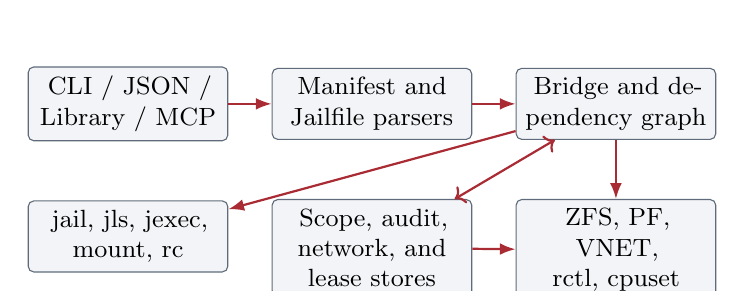
\begin{tikzpicture}[
  node distance=0.75cm and 0.55cm,
  box/.style={draw=steel,rounded corners=2pt,fill=codeback,minimum height=0.75cm,
              text width=2.3cm,align=center,font=\small},
  arrow/.style={-{Latex[length=2mm]},thick,color=signalred}
]
  \node[box] (cli) {CLI / JSON / Library / MCP};
  \node[box,right=of cli] (manifest) {Manifest and Jailfile parsers};
  \node[box,right=of manifest] (bridge) {Bridge and dependency graph};
  \node[box,below=of manifest] (state) {Scope, audit, network, and lease stores};
  \node[box,below=of cli] (freebsd) {jail, jls, jexec, mount, rc};
  \node[box,below=of bridge] (host) {ZFS, PF, VNET, rctl, cpuset};
  \draw[arrow] (cli) -- (manifest);
  \draw[arrow] (manifest) -- (bridge);
  \draw[arrow] (bridge) -- (host);
  \draw[arrow] (bridge) -- (freebsd);
  \draw[arrow,<->] (bridge) -- (state);
  \draw[arrow] (state) -- (host);
\end{tikzpicture}
\end{shipfigure}

The CLI is intentionally thin. The same core abstractions back ephemeral
library containers and long-lived manifest jails. Errors retain typed causes at
the library boundary and stable codes at the JSON boundary.

\section{Manifest, service, and project names}

The manifest is a desired-state document. Each \setting{[[jails]]} table has a
short service name. Blackship prefixes that name with the project name when it
creates the kernel jail, avoiding collisions between projects. Commands accept
the short name, the full name, an unambiguous prefix, a matching tag, or
\command{ALL} where a selector is allowed.

Dependencies form a directed acyclic graph. Starting a target walks its
prerequisites in topological order. Stopping a target normally walks its
dependents in reverse order. A cycle or unknown dependency is a configuration
error, not an ordering guess.

\section{Releases, roots, and images}

A \emph{release} is a complete FreeBSD userland that can seed a jail. It may
come from official distribution archives, pkgbase, or \command{blackship
commit}. A jail root is a writable instance of that release.

With ZFS, the release dataset owns a \command{@pristine} snapshot and jail
roots are clones. Without ZFS, Blackship copies the release directory. A
Jailfile modifies a root in reproducible steps; on ZFS, each completed
\command{RUN} or \command{COPY} can become a cached layer snapshot.

\section{Lifecycle and state machines}

The lifecycle distinguishes declared intent from partial host reality. A jail
moves through creation, startup, running, draining, stopping, cleanup, and
failure states. Blackship checkpoints ownership before each external mutation.
Consequently, cleanup can reason about a half-created interface or mount even
when no running jail exists.

The main lifecycle operations are:

\begin{description}
  \item[up] provision and start selected jails with their dependencies;
  \item[down] drain and stop selected jails in dependency-safe order;
  \item[restart] perform the stop and start plans;
  \item[eva] reconcile live-safe parameters, resource rules, and CPU placement
    without restarting; and
  \item[gc] compare durable ownership with live host state and reclaim or report
    leftovers.
\end{description}

\subsection*{One chart for lifecycle and health}

Lifecycle and health share a single statechart, so the order in which states
are left and entered is resolved by the chart instead of by hand:

\begin{figure}[htbp]
\centering
\begin{tikzpicture}[
  font=\small,
  leaf/.style={draw=steel,rounded corners=3pt,fill=codeback,minimum width=2.0cm,
               minimum height=0.8cm,align=center},
  group/.style={draw=steel,rounded corners=6pt,inner sep=0.25cm},
  title/.style={font=\footnotesize\bfseries,text=signalred,anchor=north west},
  move/.style={-{Latex[length=2mm]},thick,color=signalred},
  tag/.style={font=\footnotesize\ttfamily,text=voidblack,fill=white,inner sep=1pt}
]
  \node[leaf] (stopped)  at (1.7,5.0) {Stopped};
  \node[leaf] (failed)   at (1.7,1.4) {Failed};
  \node[leaf] (starting) at (5.9,5.0) {Starting};
  \node[leaf] (stopping) at (5.9,1.4) {Stopping};
  \node[leaf] (draining) at (10.6,1.4) {Draining};
  \node[leaf,fill=white] (healthy)   at (9.6,5.6) {Healthy};
  \node[leaf,fill=white] (unhealthy) at (11.7,5.6) {Unhealthy};
  \node[leaf,fill=white] (failing)   at (9.6,4.3) {Failing};
  \node[leaf,fill=white] (suspended) at (11.7,4.3) {Suspended};
  \coordinate (dtop) at (1.7,5.85);
  \coordinate (utop) at (8.0,7.0);
  \coordinate (jtop) at (7.0,7.6);
  \coordinate (rtl) at (8.35,6.7);
  \coordinate (rbr) at (12.95,3.65);

  \begin{scope}[on background layer]
    \node[group,fill=plasma!14,fit=(starting)(stopping)(draining)(utop)(rtl)(rbr)] (up) {};
    \node[group,fill=plasma!14,fit=(stopped)(failed)(dtop)] (down) {};
    \node[group,draw=voidblack,fit=(down)(up)(jtop),inner sep=0.3cm] (jail) {};
    \node[group,fill=ash!55,inner sep=0pt,fit=(rtl)(rbr)] (running) {};
  \end{scope}
  \foreach \bx/\name in {jail/Jail,down/Down,up/Up,running/Running}
    \node[title] at ([shift={(0.15,-0.1)}]\bx.north west) {\name};

  \draw[move] (stopped) -- node[tag,above] {start} (starting);
  \draw[move] (starting.east) -- node[tag,above] {started} (running.west |- starting.east);
  \draw[move] (draining.north |- running.south) -- node[tag,right] {drain} (draining.north);
  \draw[move] ($(running.south west)+(0.4,0)$) -- node[tag,above left] {stop} (stopping.north east);
  \draw[move] (draining.west) -- node[tag,above] {stop} (stopping.east);
  \draw[move] (stopping.north west) -- node[tag,above right,pos=0.45] {stopped} (stopped.south east);
  \draw[move] (failed.north) -- node[tag,right] {recover} (stopped.south);
  \draw[move] (up.west |- failed.east) -- node[tag,above] {fail} (failed.east);
\end{tikzpicture}
\caption{The jail chart. Arrows are the \setting{state-machines} events, with
\texttt{fail} leaving any state inside Up. The four Running leaves move among
themselves with supervisor health verdicts.}
\label{fig:jail-chart}
\end{figure}

Events and guards stay in the \setting{state-machines} jail machine; the chart
only answers which states a move exits (innermost first) and enters (outermost
first). A \command{fail} from a healthy running jail exits Healthy, Running and
Up, then enters Down and Failed. Health verdicts from the supervisor move the
leaf inside Running. When a jail stops, the claims held by Up (the VNET
interface, then the address lease) are released in the order the resolved exit
reports.

\section{Durable stores}

Files beneath the configured data directory serve different purposes:

\begin{shiptable}{L{0.22\textwidth}L{0.68\textwidth}}
\toprule
Store & Role \\
\midrule
Scope & Current ownership and the rollback work-list for a jail. \\
Audit & Append-only JSONL lifecycle history that survives scope deletion. \\
Networks & Persistent named-network definitions, recreated after reboot. \\
Leases & Serialized address ownership for concurrent jail creation. \\
Port forwards & PF mappings that can be reloaded after PF restart. \\
Container registry & Process ownership records for ephemeral library/CLI
containers, including explicit ownership handoff. \\
\bottomrule
\end{shiptable}

Mutable TOML state is staged in a uniquely named temporary file beside its
target and then atomically renamed into place. Keeping the temporary and target
files on one filesystem prevents readers from observing a partially written
scope, network, lease, forward, or container-ownership record.

\section{Failure model}

Host operations can fail between any two syscalls. Blackship therefore avoids
the fiction that a multi-step jail start is atomic. It instead makes rollback
explicit and idempotent. A failed start removes resources it created; a later
\command{cleanup} or \command{gc} can finish the work after interruption.

Resource-limit and VNET attachment failures are fatal. Running a jail after an
isolation control failed would violate the manifest more seriously than
returning an error.

\begin{shipnote}[Inspect before applying]
The structured dry-run plans are calculated from the same dependency and drift
logic used by real operations. Use \command{--format json ... --dry-run} in a UI
or \command{--dry-run} at the terminal before broad changes.
\end{shipnote}

\chapter{Getting Started}
\label{ch:getting-started}

This chapter builds a small VNET web jail backed by ZFS. The examples assume a
pool named \command{zroot}, an external interface already configured by the
host, and a FreeBSD 15.1 host.

\section{Create a project}

Make a working directory and generate a starter manifest:

\begin{lstlisting}[language=bash]
mkdir -p ~/jails/web-stack
cd ~/jails/web-stack
blackship armada init
\end{lstlisting}

Replace the generated content with a minimal configuration:

\begin{lstlisting}[language=TOML]
[config]
data_dir = "/var/blackship"
zfs_enabled = true
zpool = "zroot"
dataset = "blackship"

[[jails]]
name = "web"
release = "15.1-RELEASE"
hostname = "web.internal"

[jails.network]
vnet = true
networks = ["default"]
ip = "10.0.1.10"

[jails.healthcheck]
enabled = true

[[jails.healthcheck.checks]]
name = "nginx"
command = "service nginx status"
target = "jail"
interval = 30
timeout = 10
retries = 3
\end{lstlisting}

\section{Bootstrap the userland}

\begin{lstlisting}[language=bash]
blackship bootstrap 15.1-RELEASE
blackship releases list
\end{lstlisting}

On FreeBSD 16 and newer, official distribution sets are no longer the normal
source and Blackship uses fingerprint-verified pkgbase automatically.
\command{--pkgbase} opts into that path on supported earlier branches.

\section{Create the named network}

The default epair backend uses an \command{if\_bridge}:

\begin{lstlisting}[language=bash]
blackship network create default \
  --subnet 10.0.1.0/24 \
  --gateway 10.0.1.1 \
  --bridge blackship0
\end{lstlisting}

To use netgraph instead, choose a distinct bridge name:

\begin{lstlisting}[language=bash]
blackship network create default \
  --subnet 10.0.1.0/24 \
  --gateway 10.0.1.1 \
  --backend netgraph \
  --bridge ngbridge0
\end{lstlisting}

Do not create both examples under the same network name. Chapter
\ref{ch:networking-storage} explains the backend tradeoffs and host routing.

\section{Validate and preview}

\begin{lstlisting}[language=bash]
blackship check
blackship up web --dry-run
blackship --format json up web --dry-run
\end{lstlisting}

The plan should identify the full jail name, root path, address, hook counts,
current state, and whether a ZFS dataset will be created. Resolve every
validation error before continuing.

\section{Start and inspect the jail}

\begin{lstlisting}[language=bash]
blackship up web
blackship ps
blackship exec web -- uname -a
blackship console web
\end{lstlisting}

Install and enable a service inside the jail:

\begin{lstlisting}[language=bash]
blackship exec web -- pkg install -y nginx
blackship exec web -- sysrc nginx_enable=YES
blackship exec web -- service nginx start
blackship health web
\end{lstlisting}

For a reproducible service image, put those installation steps in a Jailfile
instead of treating the running jail as the build record; see Chapter
\ref{ch:images}.

\section{Publish a port}

PF anchors isolate Blackship-managed redirects from the rest of the host's PF
configuration:

\begin{lstlisting}[language=bash]
blackship expose web --port 8080 --internal 80
blackship ports web
\end{lstlisting}

The host PF configuration must load Blackship's anchors. A typical
\file{/etc/pf.conf} contains:

\begin{lstlisting}
rdr-anchor "blackship"
anchor "blackship"
\end{lstlisting}

Run \command{blackship setup} after a PF restart, or at boot through the
provided rc integration, to reapply persisted networks and forwards.

\section{Stop and remove resources}

\begin{lstlisting}[language=bash]
blackship down web --dry-run
blackship down web
\end{lstlisting}

\command{down} stops the running jail and releases runtime resources while
preserving its root for future starts. Use \command{rm --volumes} only when the
jail and its associated storage should be removed.

\begin{shipwarning}[Destructive cleanup]
\command{snapshot rollback --force}, \command{rm --volumes}, forced garbage
collection, release deletion, and recursive ZFS destruction can discard data.
Take a snapshot or export first, verify the resolved full jail and dataset names,
and prefer Blackship commands over manual host deletion.
\end{shipwarning}

\section{Next steps}

Add a database service with \setting{depends\_on = ["database"]}, move package
installation into a Jailfile, configure a health-driven QoS transition, and run
\command{blackship supervise}. Those features are developed in the following
chapters.

\chapter{Configuration Reference}
\label{ch:configuration}

Blackship reads TOML from \file{blackship.toml} by default. Select another file
with the global \command{--config} option. Armada can merge several manifests in
order; later files override earlier values.

\section{Global configuration}

\begin{lstlisting}[language=TOML]
[config]
project = "orbital"
data_dir = "/var/blackship"
releases_dir = "/var/blackship/releases"
cache_dir = "/var/cache/blackship"
mirror_url = "https://download.freebsd.org/releases"
zfs_enabled = true
zpool = "zroot"
dataset = "blackship"
bootstrap_archives = ["base", "lib32"]
usage_sample_secs = 30
monitor_ping_url = "https://monitor.example/ping/token"
\end{lstlisting}

\begin{shiptable}{L{0.23\textwidth}L{0.18\textwidth}L{0.49\textwidth}}
\toprule
Key & Typical value & Meaning \\
\midrule
\setting{project} & string & Prefix for effective jail names. If omitted,
Blackship uses the manifest directory name, then the working-directory name,
with a path-derived Black Ship name as the final fallback. \\
\setting{data\_dir} & path & Persistent state, roots, scopes, audit, networks,
leases, and forward records. \\
\setting{releases\_dir} & path & Bootstrapped and committed release roots. \\
\setting{cache\_dir} & path & Downloads and reusable build material. \\
\setting{mirror\_url} & URL & Base URL for FreeBSD release acquisition. \\
\bottomrule
\end{shiptable}

\begin{shiptable}{L{0.23\textwidth}L{0.18\textwidth}L{0.49\textwidth}}
\multicolumn{3}{l}{\textit{Global configuration (continued)}} \\[0.35em]
\toprule
Key & Typical value & Meaning \\
\midrule
\setting{zfs\_enabled} & boolean & Enable dataset-backed provisioning and ZFS features. \\
\setting{zpool} & string & Pool containing the Blackship dataset tree. \\
\setting{dataset} & string & Dataset path below the pool. \\
\setting{bootstrap\_archives} & array & Release components to acquire; the
default is \setting{["base"]}. \\
\setting{usage\_sample\_secs} & integer & Supervisor racct and telemetry sample
period; zero disables sampling. \\
\setting{monitor\_ping\_url} & URL & Optional dead-man ping used by the supervisor. \\
\bottomrule
\end{shiptable}

When ZFS is enabled, the jails dataset is mounted at the configured data
directory's \file{jails} path. This keeps effective root paths consistent
between directory and dataset deployments.

Operational defaults are tunable in nested tables. The following example also
shows bridge VLAN filtering, which requires FreeBSD 15.0 or newer:

\begin{lstlisting}[language=TOML]
[config.rate_limit]
jail_start_capacity = 3.0
health_capacity = 5.0
health_refill_rate = 0.5

[config.health]
interval = 30
timeout = 10
start_period = 60
retries = 3

[config.retry]
base_delay_ms = 1000
max_delay_ms = 30000
multiplier = 2.0
max_attempts = 5
jitter_factor = 0.25

[config.bridge]
name = "vswitch1"
vlan_filtering = true

[config.bridge.trunk]
interface = "igb1"
tagged = [10, 20, 99]
disable_hwfilter = false
\end{lstlisting}

Rate limits bound concurrent starts and health-check dispatch. The
\setting{config.health} schema records the intended global check defaults; in
version 0.3.0, checks use their own values or the same built-in defaults shown
above. Retry values control exponential backoff for HTTP release operations;
jitter is expressed as a fraction from zero through one. The optional trunk
block declares the physical interface and VLANs admitted by a filtering bridge.

\section{Jail definitions}

Each service is an array entry:

\begin{lstlisting}[language=TOML]
[[jails]]
name = "api"
release = "15.1-RELEASE"
hostname = "api.internal"
depends_on = ["database", "cache"]
tags = ["web", "production"]
devfs_ruleset = 4
init = true
stop = "service api stop"
ephemeral = false
\end{lstlisting}

\setting{name} is required and must be safe for a FreeBSD jail name.
\setting{release} selects the seed userland. \setting{path} may replace the
default root path, and \setting{build} or \setting{jailfile} can point Armada at
a build context. \setting{hostname} defaults from the service name.

\setting{depends\_on} defines graph edges. \setting{tags} groups several jails
under a selector. \setting{init = true} runs the FreeBSD rc lifecycle. A
manifest \setting{stop} command overrides the Jailfile's \command{STOP}.

Additional jail parameters are accepted in \setting{params}, but identity and
isolation keys managed by Blackship---including name, path, VNET, securelevel,
devfs, address, and related \command{allow.*} controls---cannot be overridden
through an escape hatch. Use first-class configuration where provided.

\section{Resource controls}

\begin{lstlisting}[language=TOML]
[jails.resources]
memory = "2g"
vmemory = "4g"
cpu = "200"
maxproc = 512
maxthreads = 1024
openfiles = 4096
swap = "1g"
cores = 2
# cpuset = "0,1"
# rules = ["readbps:deny=50m/s"]
\end{lstlisting}

Named fields become rctl rules. \setting{cpu} is percentage-style pcpu policy;
values above 100 permit more than one core of aggregate CPU. \setting{cores}
asks Blackship to choose the least-loaded CPUs while \setting{cpuset} pins an
explicit list and wins when both are present. The \setting{rules} array accepts
advanced raw RCTL resource/action expressions; a jail subject is added when
omitted, and a rule targeting a different jail is rejected.

RCTL amount fields accept integers or binary size suffixes
\setting{k}, \setting{m}, \setting{g}, \setting{t}, \setting{p}, and
\setting{e}, optionally followed by \setting{b}. Blackship expands these to
the integer form required by the kernel before issuing the rule syscall.

If configured resource enforcement cannot be applied, startup fails and rolls
back. This avoids silently running a workload beyond its declared boundary.

\section{Network configuration}

\begin{lstlisting}[language=TOML]
[jails.network]
vnet = true
networks = ["frontend"]
ip = "10.20.0.15"
# ip_cidr = "10.20.0.15/24" # alternative with explicit prefix
gateway = "10.20.0.1"
mac_address = "58:9c:fc:00:20:15"
vlan_id = 20
backend = "epair"

[jails.network.dns]
mode = "custom"
nameservers = ["10.20.0.53", "1.1.1.1"]
search = ["internal.example"]
domain = "internal.example"
\end{lstlisting}

A named network supplies subnet, bridge, gateway, and backend runtime data.
Explicit values on the jail refine that attachment. Use \setting{ip\_cidr}
when the prefix must travel with the address, or omit both address keys to use
the network lease allocator. Omit \setting{mac\_address} for a deterministic
address derived from the jail name and bridge. The backend may be
\setting{epair} or \setting{netgraph}; VLAN PVIDs are supported by the epair
backend on a filtering bridge.

Set \setting{shared = true} for host-network inheritance instead of VNET. This
is a weaker isolation mode and is ignored when VNET is enabled.

DNS mode \setting{inherit} copies the host resolver configuration. Mode
\setting{custom} writes the declared nameservers, optional search list, and
domain into the jail.

\section{Health checks}

All checks are command-oriented: exit zero passes and non-zero fails. The
target determines whether the command runs on the host or inside the jail.

\begin{lstlisting}[language=TOML]
[jails.healthcheck]
enabled = true

[[jails.healthcheck.checks]]
name = "http"
command = "fetch -qo /dev/null http://127.0.0.1:8080/health"
target = "jail"
start_period = 60
interval = 30
timeout = 10
retries = 3

[[jails.healthcheck.checks]]
name = "listener"
command = "nc -z 127.0.0.1 8080"
target = "jail"
\end{lstlisting}

The supervisor retains failure history, applies configured recovery behavior,
and can use health as the trigger for a QoS phase transition.

\section{Hooks}

\begin{lstlisting}[language=TOML]
[[jails.hooks]]
phase = "pre_start"
target = "host"
command = "/usr/local/bin/fetch-secrets"
args = ["${jail_name}"]
on_failure = "abort"

[[jails.hooks]]
phase = "pre_stop"
target = "jail"
command = "/usr/sbin/service"
args = ["nginx", "stop"]
on_failure = "continue"
\end{lstlisting}

A hook executes \setting{command} directly with \setting{args} as its argument
vector; there is no shell, so \setting{command = "service nginx stop"} names a
program that does not exist. Use \setting{command = "/bin/sh"} with
\setting{args = ["-c", "..."]} when shell syntax is needed. Arguments expand
\setting{\$\{jail\_name\}}, \setting{\$\{jail\_path\}},
\setting{\$\{jail\_ip\}}, and \setting{\$\{jid\}}.

Supported lifecycle phases include \setting{pre\_create},
\setting{post\_create}, \setting{pre\_start}, \setting{post\_start},
\setting{pre\_stop}, \setting{post\_stop}, \setting{pre\_eva}, and
\setting{post\_eva}. A phase that requires a running jail is rejected when no
JID is available. A \setting{post\_start} hook runs after the jail is up, so
\setting{abort} there only warns: the jail keeps running. Use
\setting{continue} only when failure is genuinely safe to ignore.

\section{Two-phase QoS}

\begin{lstlisting}[language=TOML]
[jails.qos]
transition = "healthy"
max_startup_secs = 120

[jails.qos.startup]
memory = "4g"
cpu = "400"

[jails.qos.steady]
memory = "2g"
cpu = "200"
\end{lstlisting}

\setting{transition} may be \setting{healthy}, \setting{timer}, or
\setting{manual}. Health-driven transition requires the supervisor;
\setting{max\_startup\_secs} provides a deadline fallback. The current phase is
recorded so EVA reconciles against it rather than reverting to startup policy.

\section{Draining and cascade policy}

A drain policy blocks new TCP connections through a jail-specific PF
sub-anchor, then waits up to its timeout for established states to close before
teardown. This is useful for service upgrades behind a load balancer.

\begin{lstlisting}[language=TOML]
[jails.drain]
enabled = true
timeout_secs = 30
\end{lstlisting}

Set \setting{cascade = "strict"}, \setting{"detach"}, or
\setting{"isolate"} on the jail entry to control dependents during
\command{down}:

\begin{description}
  \item[strict] stop dependents first; this is the default;
  \item[detach] stop only the selected target; and
  \item[isolate] leave dependents running but fence them from the stopped target.
\end{description}

\section{Telemetry}

\begin{lstlisting}[language=TOML]
[telemetry]
endpoint = "http://127.0.0.1:4318"
service_name = "blackship"
metrics_interval_secs = 30

[telemetry.headers]
authorization = "Bearer replace-me"
\end{lstlisting}

When compiled with telemetry support, the block enables OTLP/HTTP lifecycle
events and resource gauges. An unavailable collector warns but does not fail a
jail operation. Do not commit credentials in a shared manifest; merge a
protected local override when necessary.

\section{Validation discipline}

Always run both syntax/semantic validation and a lifecycle preview:

\begin{lstlisting}[language=bash]
blackship check
blackship armada config --show
blackship up --all --dry-run
\end{lstlisting}

The first catches manifest and dependency errors, the second reveals merged
Armada configuration, and the third resolves actual operational ordering.

\chapter{Releases, Jailfiles, and Images}
\label{ch:images}

Blackship separates the base FreeBSD userland from application-specific image
construction. Releases are reusable roots; Jailfiles describe deterministic
changes; a running or built jail can be committed back into another release.

\section{Bootstrapping releases}

\begin{lstlisting}[language=bash]
blackship bootstrap 15.1-RELEASE
blackship bootstrap 15.1-RELEASE --archives base,lib32
blackship bootstrap 15.1-RELEASE --pkgbase
blackship releases list
blackship releases verify 15.1-RELEASE
\end{lstlisting}

FreeBSD 16 and newer use pkgbase automatically. For pkgbase, repository
metadata is checked through the FreeBSD fingerprint trust chain. With ZFS, a
successful bootstrap creates a release dataset and \command{@pristine}
snapshot. Blackship refuses to treat an incomplete root as a valid release.

\section{Line-oriented Jailfiles}

The default format deliberately resembles a Dockerfile while retaining
FreeBSD semantics:

\begin{lstlisting}[language=Jailfile]
FROM 15.1-RELEASE
LABEL service=web version=1.0
ARG NGINX_VERSION=1.30
ENV NGINX_VERSION=${NGINX_VERSION}
RUN pkg install -y nginx
RUN sysrc nginx_enable=YES
COPY nginx.conf /usr/local/etc/nginx/nginx.conf
COPY public/ /usr/local/www/nginx/
WORKDIR /usr/local/www/nginx
EXPOSE 80/tcp
CMD /usr/local/sbin/nginx -g 'daemon off;'
STOP /usr/local/sbin/nginx -s quit
\end{lstlisting}

\begin{shiptable}{L{0.17\textwidth}L{0.73\textwidth}}
\toprule
Instruction & Meaning \\
\midrule
\command{FROM} & Required base release or committed image. \\
\command{LABEL} & Image metadata. \\
\command{ARG} & Build-time variable with an optional default. \\
\command{ENV} & Environment metadata available to later instructions. \\
\command{RUN} & Command executed while building the jail root. \\
\command{COPY} & Copy from the bounded build context into the jail root. \\
\command{WORKDIR} & Set/create the working directory for later steps. \\
\command{EXPOSE} & Document an intended service port; it does not create PF rules. \\
\command{CMD} & Default image command metadata. \\
\command{STOP} & Command run before rc shutdown; manifest \setting{stop} wins. \\
\bottomrule
\end{shiptable}

Source resolution refuses absolute paths and parent traversal. Destination
writes refuse symlink escapes from the jail root. Ownership is resolved against
the jail, not the host.

\section{TOML Jailfiles}

The alternative format is convenient for generated configuration:

\begin{lstlisting}[language=TOML]
[metadata]
name = "web"
version = "1.0"

from = "15.1-RELEASE"

[[args]]
name = "NGINX_VERSION"
default = "1.30"

[[instructions]]
type = "run"
command = "pkg install -y nginx"

[[instructions]]
type = "copy"
src = "nginx.conf"
dest = "/usr/local/etc/nginx/nginx.conf"

[[expose]]
port = 80
protocol = "tcp"

cmd = "/usr/local/sbin/nginx -g 'daemon off;'"

[stop]
cmd = "/usr/local/sbin/nginx -s quit"
\end{lstlisting}

Generate either form with \command{blackship init}; pass \command{--toml} for
the structured variant.

\section{Build, inspect, and validate}

\begin{lstlisting}[language=bash]
blackship template validate Jailfile
blackship template inspect Jailfile
blackship build --file Jailfile --name web --dry-run
blackship build --file Jailfile --name web \
  --build-arg NGINX_VERSION=1.30
\end{lstlisting}

Dry run does not bootstrap a missing release or mutate storage. Validation
should be part of CI before a privileged build job.

\section{ZFS layer cache}

Every cacheable \command{RUN} and \command{COPY} contributes to a rolling hash
of the base release, earlier instructions, build arguments, and copied content.
A completed step is snapshotted as \command{bs-layer-N-hash}. A rebuild finds
the longest matching prefix, rolls back to it, and resumes at the first changed
step.

Changing an early instruction invalidates it and all later layers. Changing an
unrelated file outside a \command{COPY} source does not. This makes build
contexts both faster and more predictable than timestamp-only caching.

\section{Commit and reuse}

\begin{lstlisting}[language=bash]
blackship build --file runner/Jailfile --name runner
blackship commit runner runner-golden
blackship run --name ci-42 --release runner-golden -- ./run-tests.sh
\end{lstlisting}

Commit stages the known jail definition and Jailfile under
\file{.blackship/}, snapshots the root, clones it into the release tree, and
promotes it so the result is independently reusable. Choose immutable,
meaningful release names; consumers should not need to know whether the seed
came from FreeBSD or a committed image.

\section{Armada build references}

\begin{lstlisting}[language=TOML]
[[jails]]
name = "web"
build = "./web"
depends_on = ["database"]

[[jails]]
name = "worker"
jailfile = "./worker/Worker.jailfile"
\end{lstlisting}

\setting{build} names a directory containing \file{Jailfile};
\setting{jailfile} names an explicit file. Armada's \command{up} builds missing
roots by default, \command{--build} forces a rebuild, and
\command{--no-build} fails when a required root does not already exist.

\begin{shipnote}[Builds are not runtime configuration]
Put packages, files, and service enablement in a Jailfile. Put host attachment,
resource policy, addresses, dependencies, and operational hooks in the
manifest. Keeping the boundary clear makes images reusable and manifests
auditable.
\end{shipnote}

\chapter{Networking and Storage}
\label{ch:networking-storage}

\section{VNET backends}

A VNET jail owns its network stack. Blackship can attach that stack through two
native FreeBSD dataplanes:

\begin{shiptable}{L{0.25\textwidth}L{0.30\textwidth}L{0.30\textwidth}}
\toprule
Property & epair backend & netgraph backend \\
\midrule
Host switching & \command{if\_bridge} & \command{ng\_bridge} node \\
Jail interface & epair peer & \command{ng\_eiface} \\
Gateway location & bridge interface & host-side \command{ng\_eiface} \\
VLAN filtering & supported on capable kernels & not supported \\
Default & yes & no \\
\bottomrule
\end{shiptable}

Create a persisted named network rather than manually creating only a bridge:

\begin{lstlisting}[language=bash]
blackship network create frontend \
  --subnet 10.20.0.0/24 \
  --gateway 10.20.0.1 \
  --backend epair \
  --bridge blackship0
\end{lstlisting}

The record survives reboot; transient interfaces do not. \command{blackship
setup} realizes missing bridges and gateway interfaces from the record.

\section{Netgraph topology}

For a netgraph network, one host-side eiface carries the gateway and each jail
receives another eiface on a free \command{linkN} hook:

\begin{shipfigure}
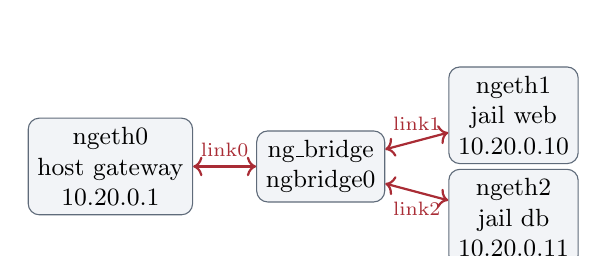
\begin{tikzpicture}[
  n/.style={draw=steel,fill=codeback,rounded corners,align=center,font=\small},
  a/.style={-{Latex[length=2mm]},thick,color=signalred},node distance=0.8cm]
  \node[n] (bridge) {ng\_bridge\\ngbridge0};
  \node[n,left=of bridge] (host) {ngeth0\\host gateway\\10.20.0.1};
  \node[n,right=of bridge,yshift=0.65cm] (web) {ngeth1\\jail web\\10.20.0.10};
  \node[n,right=of bridge,yshift=-0.65cm] (db) {ngeth2\\jail db\\10.20.0.11};
  \draw[a,<->] (host) -- node[above,font=\scriptsize]{link0} (bridge);
  \draw[a,<->] (bridge) -- node[above,font=\scriptsize]{link1} (web);
  \draw[a,<->] (bridge) -- node[below,font=\scriptsize]{link2} (db);
\end{tikzpicture}
\end{shipfigure}

Outbound traffic, on either backend, requires host forwarding and a PF NAT
rule. Blackship enables forwarding while realizing a gateway but installs no
NAT: egress belongs in the host PF policy, on the interface carrying the
default route. Without it, jails reach the gateway and each other, and nothing
else:

\begin{lstlisting}
nat on $ext_if inet from 10.20.0.0/24 to any -> ($ext_if)
\end{lstlisting}

\subsection{Bridge-name collision}

Loading \command{ng\_ether} creates netgraph nodes for ethernet interfaces,
including \command{if\_bridge} devices. An epair network named
\command{blackship0} can therefore occupy that name in both namespaces. Use a
different name such as \command{ngbridge0} for an actual netgraph bridge.

\section{Address and interface ownership}

Address claims are serialized in the lease store, so concurrent creators cannot
receive the same IP. Host-side interfaces are placed in the
\command{blackship} interface group. Cleanup verifies group ownership before
destroying an interface found by name, protecting an unrelated interface after
name reuse.

The default MAC uses FreeBSD's OUI plus a stable hash of jail and bridge names.
It survives restart while differing between clones. Explicitly configure a MAC
only when an external network policy requires it.

\section{Resolver behavior for ephemeral runs}

An ephemeral \command{run} without \command{--network} inherits the host
network stack and copies the host's \file{/etc/resolv.conf}. A run attached to
a named network receives its own VNET stack. Blackship still derives its
resolver from the host, but removes loopback nameservers and interface-scoped
link-local nameservers that the VNET stack cannot reach.

If filtering leaves no usable nameserver---commonly when the host uses
\command{local\_unbound} on \command{127.0.0.1}---creation fails instead of
starting a jail with predictably broken DNS. Supply one or more reachable
addresses explicitly:

\begin{lstlisting}[language=bash]
blackship run --name probe --release 15.1-RELEASE \
  --network frontend --dns 10.20.0.53 --dns 1.1.1.1 -- fetch https://example.com
\end{lstlisting}

The repeated \command{--dns} values replace, rather than supplement, the
host-derived nameserver list. Managed manifest jails continue to use the DNS
configuration described in Chapter~\ref{ch:configuration}.

\section{PF port forwarding}

\begin{lstlisting}[language=bash]
blackship expose web --port 443 --bind-ip 192.0.2.10
blackship expose web --port 8080 --internal 80 --proto tcp
blackship ports web
blackship unexpose web
\end{lstlisting}

Blackship writes dedicated PF anchors instead of rewriting the host ruleset.
Persisted forward definitions can be reapplied with \command{setup}. Ensure the
main ruleset contains \command{rdr-anchor "blackship"} and
\command{anchor "blackship"} before publishing a service;
\command{setup --enable-pf} writes a minimal \file{/etc/pf.conf} with both when
none exists. The \command{blackship} anchor in turn references every drain
sub-anchor, so those two lines also cover draining and \setting{isolate}.

Draining uses a per-jail sub-anchor to reject new TCP SYN packets while allowing
existing states to expire. It is not a substitute for application-level
readiness removal, but closes the race between a load balancer update and jail
teardown.

\section{ZFS layout and provisioning}

With \setting{zpool = "zroot"} and \setting{dataset = "blackship"}, Blackship
organizes release and jail datasets beneath that root. Release datasets expose a
\command{@pristine} seed; jails clone from it and mount at the same
\file{data\_dir/jails/name} path used by directory-backed roots.

Advantages include:

\begin{itemize}
  \item near-instant, copy-on-write provisioning;
  \item cheap point-in-time snapshots and clones;
  \item rolling build-layer snapshots;
  \item zero-copy commit into reusable releases; and
  \item native send/receive for backup and migration.
\end{itemize}

\section{Snapshot workflow}

\begin{lstlisting}[language=bash]
blackship snapshot create web before-upgrade
blackship exec web -- pkg upgrade -y

# Rollback requires a stopped jail.
blackship down web
blackship snapshot rollback web before-upgrade --force
blackship up web

blackship clone web@before-upgrade web-test
\end{lstlisting}

Snapshot and commit operations stage configuration under \file{.blackship/}
inside the dataset so a sent snapshot carries the metadata needed to understand
its origin.

\command{commit} promotes the new release so it no longer depends on the jail.
A side effect of \command{zfs promote}: snapshots the jail took before the
commit move to the release, and the jail can no longer roll back to them.

\section{Export, import, and migration}

\begin{lstlisting}[language=bash]
# Portable archive (bsdtar): hardlinks and file flags kept, sockets
# skipped, devfs and other mounts left out.
blackship export web --output web.tar.zst

# ZFS stream.
blackship export web --output web.zfs --zfs-send

# Restore or rename.
blackship import web.tar.zst --name web-restored

# Import a foreign jail layout.
blackship import legacy.tar --from auto --name legacy

# Move a stopped jail over SSH/ZFS receive.
blackship migrate web admin@other-host
\end{lstlisting}

A tar export is written beside its destination and renamed into place, so a
failed or interrupted export never leaves a truncated archive. Foreign import
supports iocage, ezjail, plain rootfs, or automatic detection.
Review the resulting manifest and networking before first start. Migration
requires compatible ZFS and SSH authority on the destination and does not make
an incompatible FreeBSD userland/kernel combination safe. It runs as root, so
the connection uses root's keys and \file{known\_hosts}, not the invoking
user's.

\begin{shipwarning}[Know the dataset before forcing]
Forced rollback destroys newer snapshots. Forced garbage collection or manual
\command{zfs destroy -r} can remove data Blackship cannot reconstruct. List the
resolved datasets and take an export before destructive recovery.
\end{shipwarning}

\chapter{Operations and Observability}
\label{ch:operations}

\section{Lifecycle selection and ordering}

\begin{lstlisting}[language=bash]
blackship up api
blackship up --all
blackship down production
blackship restart api
\end{lstlisting}

Selectors can be exact service names, full names, unambiguous prefixes, tags,
or \command{ALL}. Starting a target includes its dependencies; stopping uses the
configured cascade policy and reverse dependency order.

Preview broad actions before applying them:

\begin{lstlisting}[language=bash]
blackship restart --all --dry-run
blackship --format json restart --all --dry-run
\end{lstlisting}

\section{EVA live reconciliation}

EVA compares desired parameters with live values from \command{jls}, applies
updatable differences in one \command{jail\_set(JAIL\_UPDATE)} operation,
replaces managed rctl rules, and re-pins the cpuset. It runs pre/post EVA hooks
around the change.

\begin{lstlisting}[language=bash]
blackship eva api --dry-run
blackship eva api
\end{lstlisting}

Path, VNET mode, addresses, devfs ruleset, and other immutable identity or
isolation changes require a restart. EVA reports them but does not pretend to
apply them. A jail that is not running is skipped.

\section{Interactive and scripted access}

\begin{lstlisting}[language=bash]
blackship console api --user root
blackship exec api --user www -- id
blackship exec api --workdir /srv -e MODE=prod -- ./migrate
blackship exec api --clear-env -e HOME=/tmp -- env
blackship cp ./config.toml api:/usr/local/etc/app.toml
blackship cp api:/var/log/app.log ./app.log
\end{lstlisting}

Use \command{--} before the in-jail command so its flags are not parsed as
Blackship flags. Copy operations reject jail-to-jail transfers and path/symlink
escapes.

\section{Status, health, and statistics}

\begin{lstlisting}[language=bash]
blackship ps
blackship stats
blackship stats api
blackship health api
blackship health --watch --interval 5
blackship logs api --lines 200
blackship logs api --follow
\end{lstlisting}

Statistics aggregate per-process CPU and RSS from \command{jls} and
\command{ps} libxo JSON. Health status reflects configured checks and retry
state. \command{health} runs checks inside the jail and escalates to root.
The start period counts from the jail's recorded start, so a one-shot check on
a settled jail reports real results; within the period it reports
\setting{starting}, and a jail that is not running reports \setting{unknown}. Watch and follow modes are terminal streams; they are intentionally not
part of the single-envelope global JSON contract.

\section{Supervisor}

\command{blackship supervise} runs the warden loop. It monitors jail events,
executes health checks, applies recovery/backoff behavior, samples resource
usage, performs health-triggered QoS transitions, and can send a dead-man ping.
For boot operation, use the packaged rc script with the same manifest and data
directory as interactive administration.

The supervisor distinguishes intentional stops from failures and avoids
restarting a jail the operator deliberately took down. Each jail has an
independent one-for-one restart policy. Abnormal restarts back off from a
one-second base toward a 60-second ceiling, with jitter so simultaneous
failures do not restart in lockstep. The policy gives up when a jail exhausts
five restarts in a five-minute window rather than entering an endless failure
loop.

\section{QoS operations}

\begin{lstlisting}[language=bash]
blackship qos api --show
blackship qos api --steady
blackship qos api --startup
\end{lstlisting}

Only resources named by the target profile are swapped. Custom rules outside
the profile survive a phase transition. A one-shot \command{up} does not remain
resident to observe health; use the supervisor or switch manually.

\section{Audit history}

\begin{lstlisting}[language=bash]
blackship audit api
blackship --format json audit api
\end{lstlisting}

Audit JSONL is durable after the kernel jail, scope record, and even a reboot
are gone. The post-mortem summarizes event counts, lifetime, rollback steps,
termination reason, and sampled peak resources. Peaks are bounded by the sample
interval and are not exact continuous maxima.

\section{Orphan detection and garbage collection}

An out-of-band \command{jail -r}, crash, or hard reset can leave mounts,
interfaces, PF state, leases, rctl rules, or datasets behind. Garbage collection
compares durable scopes with live host state:

\begin{lstlisting}[language=bash]
blackship gc --dry-run
blackship gc
blackship gc --force
\end{lstlisting}

The normal mode reclaims only resources Blackship can prove it owns. Datasets
not created by Blackship and non-ephemeral jails are reported rather than
destroyed. \command{--force} expands authority and demands careful review.

\section{Telemetry}

When configured, lifecycle events and racct gauges are exported over OTLP/HTTP.
Telemetry runs out of band: collector failure emits a warning but cannot make a
jail lifecycle operation fail. This prevents observability from becoming a
control-plane dependency.

\section{Operational checklist}

Before a change window:

\begin{enumerate}
  \item run \command{blackship check};
  \item inspect \command{ps}, \command{health}, and recent \command{audit};
  \item snapshot stateful ZFS roots or take a portable export;
  \item generate the relevant dry-run plan;
  \item verify privilege mode and selected targets; and
  \item ensure an operator can access the host without depending on the jail
    being changed.
\end{enumerate}

After the change, verify health, port forwards, dependency status, and audit
termination/start records. Run a non-forced GC dry run to catch residual state.

\chapter{Command-Line Reference}
\label{ch:commands}

The exact parser generated by the installed binary is authoritative. Use
\command{blackship --help} and \command{blackship <command> --help} when an
option differs from this edition.

\section{Global options}

\begin{shiptable}{L{0.30\textwidth}L{0.60\textwidth}}
\toprule
Option & Effect \\
\midrule
\command{-c, --config <path>} & Select the manifest; default is
\file{blackship.toml}. \\
\command{-v, --verbose} & Emit additional operational diagnostics. \\
\command{--no-escalate} & Fail privileged commands rather than re-executing
through mdo, doas, or sudo. \\
\command{--non-interactive} & Add non-prompting behavior to doas/sudo; mdo is
inherently policy-based and non-interactive. \\
\command{--format text|json} & Select human text or the versioned machine
contract for supported commands. \\
\bottomrule
\end{shiptable}

Global options precede the subcommand. Use \command{--} to terminate option
parsing before an in-jail argv.

\section{Lifecycle and host commands}

\begin{shiptable}{L{0.39\textwidth}L{0.51\textwidth}}
\toprule
Command & Purpose \\
\midrule
\command{up [target] [--all] [--dry-run]} & Start selected jails with their
dependencies. \\
\command{down [target] [--all] [--dry-run]} & Stop in cascade/reverse dependency
order. \\
\command{restart [target] [--all] [--dry-run]} & Compose stop and start plans. \\
\command{eva [target] [--all] [--dry-run]} & Apply live-safe manifest drift. \\
\command{autostart [--dry-run]} & Reconcile running project jails to the
reserved \setting{autostart} tag and its dependency closure. \\
\command{ps [--host] [--json]} & List configured jail state and JID. With
\command{--host}, also include running jails outside the selected manifest. \\
\command{check} & Validate and resolve configuration; warn on releases not bootstrapped. \\
\command{capabilities} & Report binary, kernel, feature, facility, and escalator
capabilities. \\
\command{host} & Report the comprehensive host planning profile as JSON. \\
\command{setup [--enable-pf]} & Recreate networks/anchors and prepare the host;
optionally configure and start PF. \\
\command{cleanup <jail> [--force]} & Remove resources after a failed lifecycle. \\
\command{gc [jail] [--dry-run] [--force] [--prune-unreferenced]} & Find and
reclaim orphaned resources, including datasets left by a restarted jail and
empty bridges Blackship created; pruning broadens ownership beyond tracked
state. \\
\bottomrule
\end{shiptable}

\section{Execution and files}

\begin{shiptable}{L{0.39\textwidth}L{0.51\textwidth}}
\toprule
Command & Purpose \\
\midrule
\command{console <jail> [--user user]} & Open an interactive jail shell. \\
\command{exec <jail> [options] -- <argv>} & Execute a command with optional user,
working directory, and environment. \\
\command{run --name N --release R [--network NET] [--dns IP] -- <argv>} &
Run a command in an ephemeral jail, optionally overriding its repeatable
nameserver list; the jail is removed when the command exits. \\
\command{run --name N --release R [--network NET] [--dns IP] -d} &
Start an ephemeral jail and leave it running; takes no command. Use
\command{exec}, then \command{rm}. \\
\command{cp <source> <destination> [--preserve]} & Copy host-to-jail or
jail-to-host; use \command{jail:path} with a short or full jail name. \\
\command{rm <jails...> [--force] [--volumes]} & Remove ephemeral/managed jail
artifacts and optionally datasets; exits non-zero if any jail was not removed. \\
\command{logs <jail> [--follow] [--lines N]} & Read the jail log. \\
\bottomrule
\end{shiptable}

\section{Releases and builds}

\begin{shiptable}{L{0.39\textwidth}L{0.51\textwidth}}
\toprule
Command & Purpose \\
\midrule
\command{bootstrap <release> [--force] [--archives A] [--pkgbase]} & Acquire a
base userland. \\
\command{releases [list|delete|verify]} & Inspect or manage release roots. \\
\command{init [--file F] [--release R] [--toml] [--force]} & Generate a starter
Jailfile. \\
\command{build [--file F] [--name N] [--build-arg K=V] [--context D]
[--dry-run]} & Build an image root. \\
\command{template list|inspect|validate} & Work with Jailfiles and templates. \\
\command{commit <jail> <release>} & Freeze a jail into a reusable release. \\
\bottomrule
\end{shiptable}

\section{Networking and storage}

\begin{shiptable}{L{0.39\textwidth}L{0.51\textwidth}}
\toprule
Command & Purpose \\
\midrule
\command{network create <name> --subnet CIDR [options]} & Persist and realize a
named epair or netgraph network. \\
\command{network destroy <name> [--force]} & Remove a managed network. \\
\command{network list} & List managed network records and runtime state. \\
\command{expose <jail> --port P [options]} & Add a PF port forward. \\
\command{ports [jail]} & List persisted forwards. \\
\command{unexpose <jail>} & Remove a jail's forwards. \\
\command{snapshot create|list|rollback|delete} & Manage jail ZFS snapshots. \\
\command{clone <jail>@<snapshot> <name>} & Create a jail root from a snapshot. \\
\command{export <jail> [--output F] [--zfs-send]} & Produce a portable archive or
ZFS stream. \\
\command{import <file> [--name N] [--force] [--from manager]} & Restore native
or foreign jail data. \\
\command{migrate <jail> <user@host> [--remote-dataset D] [--keep]} & Send a
stopped ZFS-backed jail over SSH. \\
\bottomrule
\end{shiptable}

\section{Health and orchestration}

\begin{shiptable}{L{0.39\textwidth}L{0.51\textwidth}}
\toprule
Command & Purpose \\
\midrule
\command{health [jail] [--watch] [--interval N] [--json]} & Run configured
checks. \\
\command{stats [jail] [--json]} & Aggregate CPU, RSS, and process counts. \\
\command{supervise [--autostart]} & Run the warden for all configured jails;
the option reconciles and supervises only the effective boot set. \\
\command{qos <jail> --show|--startup|--steady} & Inspect or change a QoS phase. \\
\command{audit <jail> [--json]} & Render durable lifecycle history. \\
\command{armada init|up|down|build|ps|config} & Compose multi-jail workflows and
merged manifests. \\
\command{completion bash|elvish|fish|nu|zsh} & Generate shell completion. \\
\command{mcp [--listen ADDR:PORT]} & Serve MCP on stdio, or Streamable HTTP with \command{--listen} (token required off loopback). \\
\bottomrule
\end{shiptable}

\section{Machine-readable contract}

The global JSON format writes one versioned success object to standard output:

\begin{lstlisting}[language=JSON]
{
  "schema_version": 1,
  "ok": true,
  "data": []
}
\end{lstlisting}

Failures exit non-zero and write one object to standard error:

\begin{lstlisting}[language=JSON]
{
  "schema_version": 1,
  "ok": false,
  "error": {
    "code": "jail_not_found",
    "message": "Jail 'web' not found"
  }
}
\end{lstlisting}

Stable error codes are for program logic; messages are diagnostic. Commands
without a complete contract return \command{unsupported\_output\_format} rather
than mixing prose into JSON.

Read-only coverage includes status, validation, capabilities, the host planning
profile, networks, ports,
release listing, stats, one-shot health, audit, snapshot listing, and Armada
status. Lifecycle JSON is restricted to \command{--dry-run}. Streaming watch or
follow modes cannot fit a single response envelope.

\command{ps --host} returns the selected project and config path plus ownership
metadata for each row. It includes every manifest jail and running unmanaged
jails. Stopped unmanaged jails are not discoverable without a known manifest
and are omitted.

Legacy command-local \command{--json} flags remain unenveloped for compatibility.
New clients should prefer the global format and check
\setting{schema\_version} before decoding \setting{data}.

\section{Exit behavior}

Zero means the requested operation completed. Non-zero means parsing,
validation, escalation, host operation, or rendering failed. An in-jail
\command{exec} propagates the executed process status; treat that result as
workload data rather than a Blackship transport error in automation.

\chapter{Automation and Integration}
\label{ch:automation}

\section{Armada orchestration}

Armada is the multi-jail, compose-style interface. It can initialize a
manifest, merge several files, build missing roots, and apply lifecycle actions
to selected services.

\begin{lstlisting}[language=bash]
blackship armada init
blackship armada -f base.toml -f production.toml config --show
blackship armada -f base.toml -f production.toml up --detach
blackship armada ps
\end{lstlisting}

Later files override earlier values. Keep secrets and host-local paths in a
protected final override rather than the shared base manifest. Validate the
merged view, not only each input in isolation.

\section{JSON clients}

A management application should begin with:

\begin{enumerate}
  \item \command{blackship --format json capabilities};
  \item a schema-version check;
  \item \command{check} against the selected manifest;
  \item read-only status calls; and
  \item a structured dry run before offering an apply action.
\end{enumerate}

Invoke Blackship with a fixed executable path and explicit working directory.
Capture stdout and stderr separately. Decode the envelope only from the stream
documented for the exit case. Never parse the human message to determine an
error category.

Use \command{--no-escalate} when the parent application owns authorization, or
\command{--non-interactive} in unattended jobs. An interactive privilege prompt
inside a GUI or CI pipe is both confusing and prone to deadlock.

\section{Rust library}

The library API supports ephemeral jails without the CLI, parser, MCP server,
or telemetry runtime:

\begin{lstlisting}[language=TOML]
[dependencies]
blackship = { version = "0.2", default-features = false }
\end{lstlisting}

\begin{lstlisting}[language=Rust]
use blackship::{ContainerSpec, Exec, Host, Limits, Network, Selector};
use std::time::Duration;

let host = Host::new("/var/db/ci/blackship")
    .with_zfs("zroot", "ci/blackship");

host.reap_orphans(&Selector::prefix("job-"))?;
host.ensure_release("15.1-RELEASE")?;

let job = host.create(
    &ContainerSpec::new("job-42", "15.1-RELEASE")
        .network(Network::Inherit)
        .limits(Limits::new().memory("4g").max_processes(512)),
)?;

let result = job.exec(
    Exec::shell("make test")
        .cwd("/work")
        .env("CI", "true")
        .timeout(Duration::from_secs(900)),
)?;

job.destroy()?;
\end{lstlisting}

\command{Host} is a clonable description of layout and storage, not a remote
connection. Containers own independent host descriptions and can be used from
several threads. Dropping a container attempts cleanup; call \command{destroy}
when errors must be observed or \command{keep} when the instance should outlive
the handle.

A non-zero executed command is represented in the execution result, while
failure to create, enter, supervise, or clean the jail is a typed
\command{blackship::Error}. Library calls require appropriate privilege and
never re-execute through an escalation helper.

\section{Cargo features}

\begin{longtable}{L{0.20\textwidth}L{0.16\textwidth}L{0.54\textwidth}}
\toprule
Feature & Default & Adds \\
\midrule
\command{cli} & yes & Binary and usage parser; implies telemetry. \\
\command{mcp} & yes & MCP host, schemas, tracing, and stdio server; implies CLI. \\
\command{telemetry} & through CLI & OTLP export through rama. \\
\command{inspect} & no & State-machine introspection. \\
\bottomrule
\end{longtable}

\section{MCP server}

\command{blackship mcp} speaks Model Context Protocol over stdin/stdout. It is
an authoring and validation surface, not a privileged lifecycle daemon. Its
read-only tools expose host facts and the real manifest/Jailfile parsers.
File-producing tools render and validate a draft, then require operator
elicitation before an atomic write.

The gate fails closed: refusal, timeout, an unsupported client, missing
confirmation, a nonexistent destination directory, or failed validation leaves
no file behind. Replacing a file requires an additional overwrite decision.

MCP resources include a generated CLI manual, KDL command tree, JSON schemas,
Jailfile reference, and reserved jail-parameter reference. Because these are
generated from live code, use them when exact current syntax matters.

\section{CI pattern}

A CI adapter can map one job to one ephemeral jail:

\begin{enumerate}
  \item reap orphaned jobs with a narrow prefix or label selector;
  \item ensure the requested release or committed image exists;
  \item create a uniquely named jail and bounded mounts/resources;
  \item copy or mount the workspace;
  \item execute steps with explicit timeouts;
  \item copy reports out; and
  \item destroy the jail in a finally/defer path.
\end{enumerate}

Timeout supervision kills the workload from the host side so a process inside
the jail cannot evade it. Use read-only mounts for shared source or caches when
the job should not mutate host data.

\section{Versioning expectations}

Pin crate and binary versions in automation. Treat the JSON
\setting{schema\_version} independently from the Blackship package version.
Feature-detect optional behavior with \command{capabilities}, and never assume a
host has ZFS, PF, RCTL, or an authorized escalator solely because another host
did.

\chapter{Security and Reliability}
\label{ch:security}

\section{Security boundary}

A FreeBSD jail is operating-system-level isolation, not hardware virtualization.
It shares the host kernel. Blackship reduces configuration error and limits
resource/network exposure, but cannot strengthen a jail beyond the guarantees
of the running FreeBSD kernel and its policy.

Use a VM boundary for untrusted tenants that require independent kernels or for
workloads whose compromise impact cannot include the host kernel. Keep the host
patched and avoid granting broad jail parameters merely to make an application
work.

\section{Least privilege}

Most inspection and authoring operations are unprivileged. Host mutations need
root, and so do reads that enter a jail or its state: \command{health},
\command{logs}, and \command{gc} (even with \command{--dry-run}). An
unprivileged \command{eva --dry-run} cannot read VNET addresses or kernel
rctl rules and reports them as unverified. The CLI's escalation order is mdo, doas, then sudo, using canonical paths.
The library never escalates.

For interactive administration, define narrowly scoped \command{mac\_do} or
doas policy rather than unrestricted root shells. For a management UI, separate
the unprivileged planning process from the small authorized apply path and pass
\command{--no-escalate} to the former.

\section{Environment and path hygiene}

On mdo re-exec, Blackship resets \command{HOME}, \command{USER}, and
\command{LOGNAME} to root and removes XDG directory overrides. This prevents a
privileged invocation from continuing to use attacker-controlled user paths.

The executable and escalators should be installed in root-owned locations.
Automation should use an absolute Blackship path, a known working directory,
and an explicit manifest. Do not accept an arbitrary manifest path from an
untrusted caller and then authorize its lifecycle operations.

Jailfile copies are bounded to the build context and jail root. Symlink and
parent-directory escapes are rejected. MCP writes use a temporary file in the
target directory followed by rename, preventing an interrupted write from
truncating an existing manifest.

\section{Network policy}

VNET offers a separate network stack; shared networking does not. PF rules
still belong to the host security policy. Audit the base ruleset, NAT, Blackship
anchors, and external interface exposure together.

Port forwarding defaults should bind only where required. A service intended
for localhost should not be published on every host address. DNS and gateway
values in a manifest are configuration, not authentication.

Blackship verifies interface ownership before cleanup and serializes address
leases, reducing races and accidental deletion. Operators should nevertheless
avoid manually renaming or reusing managed interfaces while jails are active.

\section{Storage and secrets}

Jail roots, snapshots, exports, build contexts, staged manifests, and ZFS send
streams may contain secrets. Protect them according to the most sensitive jail
content. A snapshot is not sanitized because the live file was later deleted.

Keep telemetry tokens and local credentials in protected overrides. Review
Jailfiles before building: \command{RUN} is privileged application installation
inside a root filesystem and may fetch or execute external content.

Library-container nullfs mounts deserve two-sided review. Read-write mounts are
\command{nosuid} inside the jail by default and can also be made
\command{noexec}; neither property changes access through the original host
path. Put writable, user-reachable host directories on a dataset with
\command{setuid=off}. Treat \command{allow\_setuid()} and
\command{allow\_chflags()} as narrow exceptions for trusted build workloads,
not general compatibility switches.

\section{Reliability model}

Blackship records ownership before mutation and performs reverse-order rollback.
Cleanup is designed to be idempotent, because a crash can interrupt either the
forward path or rollback itself. Mutable TOML state is written to a unique
same-directory temporary file and atomically renamed over the target. Scope
records are current work-lists; audit records are durable history.

The project treats isolation failures as fatal. It does not continue after a
requested VNET attach or resource policy fails. This fail-closed behavior may
surface host misconfiguration earlier than a hand-written jail script, which is
the intended result.

\section{Safe change procedure}

\begin{enumerate}
  \item identify the exact project, target selector, and resolved full jail names;
  \item validate the manifest and merged overrides;
  \item inspect capabilities and current status;
  \item snapshot or export state that cannot be recreated;
  \item generate a dry-run plan;
  \item apply with non-interactive escalation only when credentials are already
    available;
  \item verify health and network reachability; and
  \item inspect audit and a GC dry run for residual resources.
\end{enumerate}

\section{Backup and recovery}

Test restoration, not only backup creation. A complete recovery plan includes:

\begin{itemize}
  \item the manifest and Jailfiles in version control;
  \item portable exports or replicated ZFS snapshots for mutable jail data;
  \item the pool/dataset naming expected on the destination;
  \item host PF, loader, rc, and escalation policy outside Blackship's data tree;
  \item release availability compatible with the destination kernel; and
  \item a procedure to recreate named networks and forwards with
    \command{blackship setup}.
\end{itemize}

\begin{shipwarning}[Force means proof has been relaxed]
Forced cleanup and garbage collection exist for damaged states where ownership
cannot be established normally. They are not routine shortcuts. Capture status,
scope/audit files, mounts, interfaces, PF anchors, and datasets before forcing;
that evidence is often what explains the incident.
\end{shipwarning}

\section{Auditability}

Use stable JSON error codes and audit events for automated decisions. Retain
the package version and capability report alongside incident logs. Human CLI
text is for diagnosis and may evolve; it is not a durable event schema.

\chapter{Troubleshooting}
\label{ch:troubleshooting}

Start every investigation with the non-mutating facts:

\begin{lstlisting}[language=bash]
blackship capabilities
blackship check
blackship ps
blackship up --all --dry-run
blackship gc --dry-run
\end{lstlisting}

Add \command{--verbose} for command diagnostics. Preserve audit and scope data
before manual cleanup.

\section{A jail will not start}

\begin{enumerate}
  \item run \command{check} for dependency, name, and path errors;
  \item verify the selected release with \command{releases verify};
  \item inspect the dry-run path, address, hooks, and dataset action;
  \item confirm RCTL is enabled if resources are configured;
  \item inspect named network state and required kernel modules; and
  \item run \command{cleanup <jail>} only after recording the original error.
\end{enumerate}

A VNET or resource-limit error is fatal by design. Fix the host capability or
remove the unsupported requirement; do not expect Blackship to run the jail
with weaker isolation.

\section{RCTL is unavailable}

Check the read-only loader tunable:

\begin{lstlisting}[language=bash]
sysctl kern.racct.enable
\end{lstlisting}

It cannot be enabled at runtime. Add \command{kern.racct.enable="1"} to
\file{/boot/loader.conf} and reboot. After reboot, validate the actual rules
with \command{rctl -l jail:<full-name>}.

\section{Network creation or attachment fails}

\begin{lstlisting}[language=bash]
blackship network list
ifconfig -g blackship
sysctl net.inet.ip.forwarding
pfctl -sr
pfctl -sn
\end{lstlisting}

For netgraph, inspect node names and avoid reusing an \command{if\_bridge} name.
For epair, confirm the bridge and interface modules are available. Verify that
the jail address belongs to the named subnet and is not already leased.

If outbound packets leave the jail but not the host, check forwarding and NAT.
If inbound forwarding fails, confirm both the Blackship anchor and the anchor
load statements in \file{/etc/pf.conf}; then run \command{blackship setup} after
any PF reload.

\section{The jail has no DNS}

Inspect \file{/etc/resolv.conf} inside the jail and the manifest's DNS mode.
Custom nameservers must be reachable from the jail's subnet. In inherited mode,
ensure the host resolver file existed when the root was prepared. DNS failure
with working IP connectivity is not a bridge failure.

For an ephemeral \command{run} on a named network, Blackship removes host
loopback and interface-scoped link-local nameservers because its VNET stack
cannot reach them. If the host resolver contains only such entries, creation
fails with an instruction to supply a reachable server:

\begin{lstlisting}[language=bash]
blackship run --name probe --release 15.1-RELEASE \
  --network default --dns 192.0.2.53 -- host freebsd.org
\end{lstlisting}

Use repeated \command{--dns} options for redundancy. Do not point a VNET jail
at \command{127.0.0.1} unless it runs its own resolver there.

\section{A netgraph bridge name is already in use}

\command{ng\_ether} gives ethernet interfaces netgraph node names. If an
\command{if\_bridge} named \command{blackship0} already exists, create the
netgraph network as \command{ngbridge0} or another distinct name. The two bridge
types share a naming namespace even though their switching implementations
differ.

\section{EVA reports restart-required drift}

Path, VNET, addresses, and certain jail parameters are immutable for Blackship's
live-reconciliation model. EVA reports them without applying them. Schedule:

\begin{lstlisting}[language=bash]
blackship restart <jail> --dry-run
blackship restart <jail>
\end{lstlisting}

If \command{jls} cannot report a requested key, EVA may label it unreadable and
apply an updatable desired value blind. Review that result on the host's exact
FreeBSD version.

\section{A build unexpectedly reruns steps}

The layer key includes the base release, prior instructions, build arguments,
and copied content. A change early in the Jailfile correctly invalidates later
layers. Confirm that generated files in a \command{COPY} source are stable and
that the same build arguments are supplied. Check available ZFS snapshots; the
layer cache is a ZFS feature.

\section{Snapshot rollback is refused}

Stop the jail before rollback. If newer snapshots exist, a non-forced rollback
protects them. List snapshots, export anything needed, and only then decide
whether \command{--force} is appropriate.

\section{Residual resources remain after a crash}

Run a GC dry run and compare its report with \command{mount}, \command{jls},
\command{ifconfig -g blackship}, PF anchors, rctl rules, and ZFS datasets.
Normal GC reclaims proven ownership. Use targeted \command{cleanup} for one
jail. Force only after confirming that a reported resource does not belong to a
different live workload.

\section{Automatic escalation fails}

Run the command once with \command{--no-escalate} to confirm that privilege is
the only issue. Check \command{capabilities} for installed helper paths. For
mdo, verify the applicable \command{mac\_do} rule; installation alone does not
grant authorization. For unattended execution, ensure doas/sudo policy permits
the command without a password and use \command{--non-interactive}.

\section{JSON automation receives an error}

Confirm the global option precedes the command and that the command supports the
contract. Streaming health/watch and log/follow output is not a single JSON
envelope. On failure read stderr, check \setting{ok = false}, branch on the
stable error \setting{code}, and log the message for operators.

\section{Raw sockets or chflags inside an ephemeral run}

Ephemeral \command{run} jails are intentionally not granted raw sockets,
arbitrary socket families, or chflags. Use a managed manifest jail with an
explicitly reviewed policy for workloads that require those facilities. Do not
broaden all ephemeral jobs to accommodate one diagnostic command.

\section{When to report a bug}

Include the Blackship version, \command{capabilities} output, FreeBSD release,
minimal manifest with secrets removed, exact command, verbose error, relevant
audit records, and whether ZFS/PF/RCTL/VNET are enabled. State whether the issue
reproduces after a dry-run-only invocation. Never attach private keys, tokens,
full production roots, or unsanitized ZFS streams.


\appendix
\chapter{Glossary}

\begin{description}[style=nextline]
  \item[Armada] Compose-style Blackship interface for merged manifests and
  multi-jail build/lifecycle operations.

  \item[Audit log] Append-only JSONL lifecycle history retained beyond cleanup.

  \item[Bridge] Both the internal Blackship coordinator and, in networking
  context, a FreeBSD packet-switching object. Context distinguishes them.

  \item[Cascade policy] Rule deciding whether dependents stop, detach, or are
  isolated when a dependency stops.

  \item[EVA] Live reconciliation of updatable jail parameters, rctl policy, and
  CPU placement without a jail restart.

  \item[Full jail name] Project-prefixed name registered with the FreeBSD kernel.

  \item[Jailfile] Reproducible application image recipe in line or TOML form.

  \item[Named network] Persistent Blackship record describing subnet, gateway,
  bridge, and backend; realized again after reboot.

  \item[Release] Complete FreeBSD userland or committed compatible image used to
  seed jail roots.

  \item[Scope record] Durable description of resources currently owned by one
  lifecycle, used as a rollback and reclamation work-list.

  \item[Service name] Short jail name written in the manifest.

  \item[VNET] FreeBSD virtualized network stack assigned to a jail.

  \item[Warden] Blackship supervisor responsible for health, recovery, usage
  sampling, and QoS transitions.

  \item[ZFS clone] Writable dataset created from a snapshot while sharing
  unchanged blocks with its origin.
\end{description}

\chapter{Paths and Files}

Exact paths follow \setting{data\_dir}, \setting{releases\_dir},
\setting{cache\_dir}, and XDG overrides. The table shows conceptual locations;
inspect the active manifest before recovery work.

\begin{shiptable}{L{0.36\textwidth}L{0.54\textwidth}}
\toprule
Path or file & Purpose \\
\midrule
\file{blackship.toml} & Default project manifest. \\
\file{Jailfile} / \file{Jailfile.toml} & Application image recipe. \\
\file{<data\_dir>/releases} & Directory-backed release roots or mountpoints. \\
\file{<data\_dir>/jails} & Jail roots or ZFS mountpoints. \\
\file{<data\_dir>/scope} & Per-jail ownership and rollback records. \\
\file{<data\_dir>/audit} & Durable per-jail JSONL histories. \\
\file{<data\_dir>/networks} & Named-network records. \\
\file{<data\_dir>/mcp.log} & MCP diagnostics when the server is used. \\
\file{<cache\_dir>} & Downloads and build cache material. \\
\file{<jail-root>/.blackship} & Staged jail definition and Jailfile carried by
snapshots/exports. \\
\file{/boot/loader.conf} & Boot-only RACCT enablement. \\
\file{/etc/pf.conf} & Host PF policy and Blackship anchor load points. \\
\file{/etc/rc.conf} & Host service enablement, including packaged warden setup. \\
\bottomrule
\end{shiptable}

\section*{Recovery rule}

Runtime state files are implementation records, not an alternate configuration
API. Back them up for diagnosis, but do not edit them to force desired state.
Prefer a validated manifest plus \command{eva}, \command{cleanup},
\command{setup}, or \command{gc}. If manual host repair is unavoidable, capture
the original files and audit trail first.


\backmatter
\chapter*{Colophon}
\addcontentsline{toc}{chapter}{Colophon}
This manual is authored in LaTeX and built from discrete chapter sources in
\path{docs/manual/chapters}. The cover uses original raster artwork, with its
title and edition information typeset separately by LaTeX.

Blackship is distributed under the BSD 3-Clause License. See the project
repository for source code, current release notes, and license text.

\end{document}
